% L13c figure: what runs where in an MCP system.
%
% The user's computer runs the host, the application that the user works with,
% and our two MCP servers. The host is drawn wide at the top and the servers
% below it, indented like children in a tree, because the host starts them. The
% host and the servers exchange MCP messages over stdio, so those messages stay
% on the computer. Three HTTPS connections cross the Internet to remote servers: the
% host to the LLM, the weather server to the NWS API, and the FRED server to the
% FRED API. The figure follows the stdio paragraph of the Hosts, Clients, and
% Servers section.
%
% Drawn on November 18, 2026 with the computers of the L13a client-server
% figure and the arrow colors of the L13c architecture figure. The notebook SVG
% carries a dark palette added by theme_svg.py; keep new colors in that script's
% mapping when changing the palette here.
\documentclass[tikz,border=4pt]{standalone}
\usepackage[no-math]{fontspec}
\IfFontExistsTF{Arial}{\setsansfont{Arial}}{\setsansfont{TeX Gyre Heros}}
\IfFontExistsTF{Menlo}{\setmonofont{Menlo}}{}
\renewcommand{\familydefault}{\sfdefault}
\usetikzlibrary{arrows.meta, calc, shapes.symbols}

% Ink, blue, gray, and band match the other L13c figures. Blue marks the MCP
% messages and dark ink marks HTTPS. Beige, key, screen, and phosphor draw the
% computers, as in the L13a client-server figure.
\definecolor{vnink}{HTML}{202124}
\definecolor{gdblue}{HTML}{0091FF}
\definecolor{gdgray}{HTML}{6D7278}
\definecolor{waband}{HTML}{EEF0F2}
\definecolor{pcbeige}{HTML}{E6DFC8}
\definecolor{pckey}{HTML}{CFC6AA}
\definecolor{crt}{HTML}{23302A}
\definecolor{phosphor}{HTML}{36C26A}

% A small tower computer, centered on the given point.
\newcommand{\tower}[1]{
  \begin{scope}[shift={#1}]
    \draw[part] (-0.32,-0.80) rectangle (-0.18,-0.74);
    \draw[part] (0.18,-0.80) rectangle (0.32,-0.74);
    \draw[case, rounded corners=2pt] (-0.40,-0.74) rectangle (0.40,0.74);
    \foreach \y in {0.42, 0.16} {
      \draw[part] (-0.28,\y) rectangle ++(0.56, 0.20);
      \draw[slot, line width=0.8pt] (-0.20,\y+0.10) -- ++(0.32, 0);
    }
    \draw[draw=vnink, fill=phosphor, line width=0.3pt] (-0.20,-0.04) circle (0.045);
    \draw[draw=vnink, fill=phosphor, line width=0.3pt] (-0.06,-0.04) circle (0.045);
    \draw[part] (0.20,-0.04) circle (0.07);
    \foreach \y in {-0.60, -0.47, ..., -0.20} {
      \draw[draw=vnink, line width=0.6pt, line cap=round] (-0.24,\y) -- (0.24,\y);
    }
  \end{scope}
}

\begin{document}
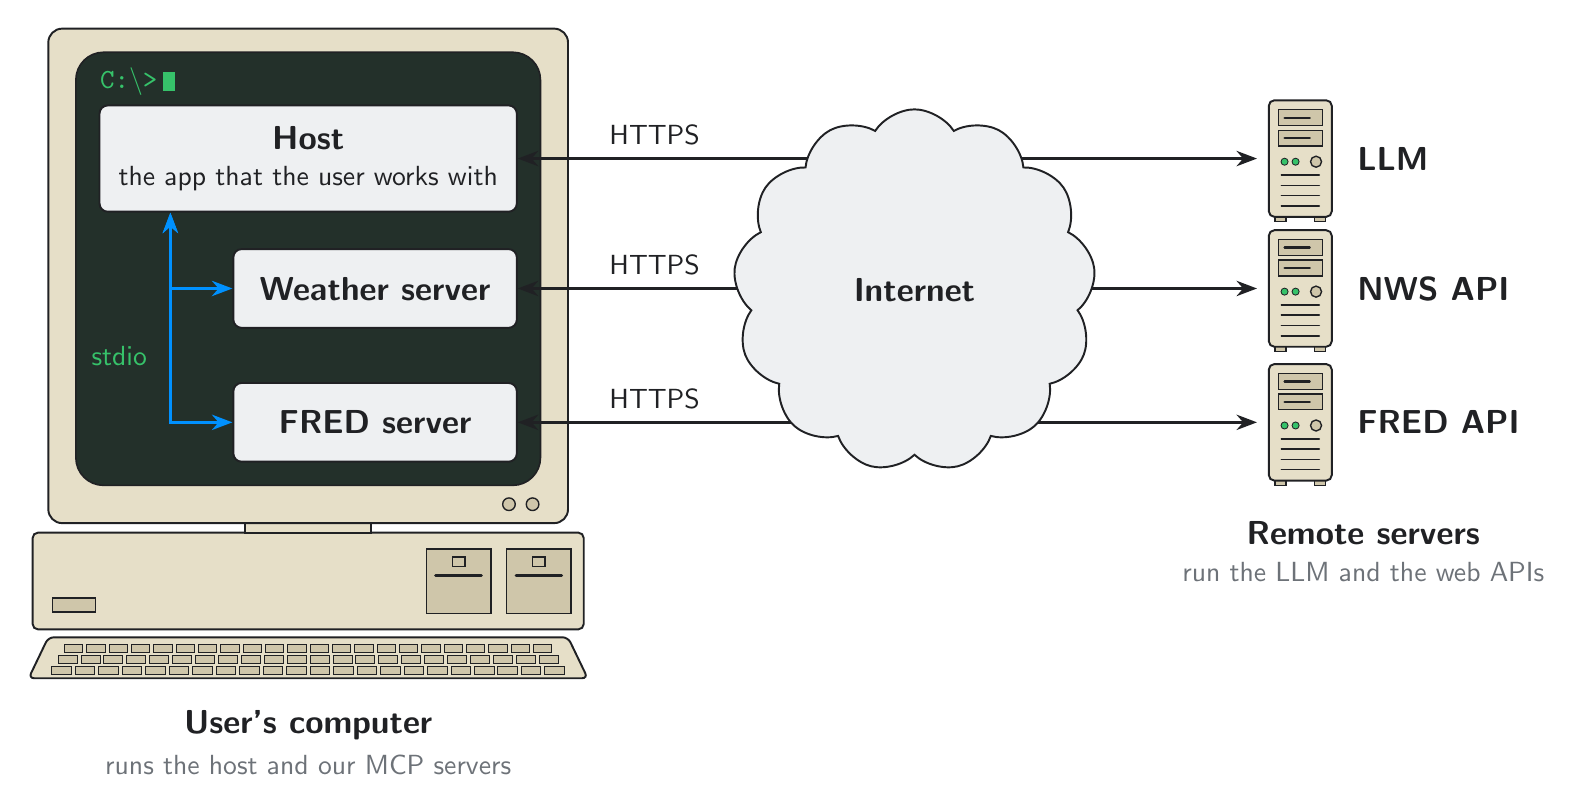
\begin{tikzpicture}[
  font=\sffamily\large,
  >={Stealth[length=2.6mm]},
  case/.style={draw=vnink, fill=pcbeige, line width=0.7pt},
  part/.style={draw=vnink, fill=pckey, line width=0.5pt},
  slot/.style={draw=vnink, line width=1.1pt, line cap=round},
  program/.style={draw=vnink, rounded corners=3pt, minimum width=3.6cm,
    minimum height=1.0cm, fill=waband, line width=0.7pt, text=vnink,
    align=center, font=\sffamily\large\bfseries},
  hostbox/.style={program, minimum width=5.3cm, minimum height=1.35cm},
  title/.style={font=\sffamily\large\bfseries, text=vnink},
  note/.style={font=\sffamily\normalsize, text=gdgray, align=center},
  msg/.style={font=\sffamily\normalsize, text=vnink},
  stdio/.style={<->, line width=1.0pt, draw=gdblue},
  https/.style={<->, line width=1.0pt, draw=vnink}
]

% ------------------------------------------- the user's computer: a desktop
% keyboard, drawn as a slab that widens toward the viewer
\draw[case, rounded corners=2pt] (-3.30,-0.98) -- (3.30,-0.98) -- (3.55,-1.50)
  -- (-3.55,-1.50) -- cycle;
\foreach \r in {0, 1, 2} {
  \pgfmathsetmacro{\half}{3.12 + 0.08*\r}
  \pgfmathsetmacro{\ytop}{-1.07 - 0.14*\r}
  \pgfmathsetmacro{\keyw}{2*\half/22}
  \foreach \k in {0, ..., 21} {
    \draw[part, line width=0.35pt] (-\half + \k*\keyw + 0.025, \ytop)
      rectangle ++(\keyw - 0.05, -0.10);
  }
}

% system unit with two floppy drives on the right
\draw[case, rounded corners=2pt] (-3.50,-0.88) rectangle (3.50,0.35);
\foreach \x in {1.50, 2.52} {
  \draw[part] (\x,-0.68) rectangle ++(0.82, 0.82);
  \draw[slot] (\x+0.12,-0.20) -- ++(0.58, 0);
  \draw[part] (\x+0.33,-0.08) rectangle ++(0.16, 0.12);
}
\draw[part] (-3.25,-0.66) rectangle (-2.70,-0.48);

% monitor on a short stand, with a dark screen and a prompt
\draw[case] (-0.80,0.35) rectangle (0.80,0.47);
\draw[case, rounded corners=5pt] (-3.30,0.47) rectangle (3.30,6.75);
\draw[draw=vnink, fill=crt, line width=0.6pt, rounded corners=10pt]
  (-2.95,0.95) rectangle (2.95,6.45);
\node[anchor=west, text=phosphor, font=\ttfamily\normalsize, inner sep=0pt]
  (prompt) at (-2.65,6.08) {C:\textbackslash>};
\fill[phosphor] ($(prompt.east)+(0.06,-0.12)$) rectangle ++(0.15, 0.24);
\draw[part] (2.55,0.71) circle (0.08);
\draw[part] (2.85,0.71) circle (0.08);

% the programs that run on the user's computer: the host, and the two servers
% that the host starts
\node[hostbox] (host) at (0.0, 5.10)
  {Host\\[-1pt]{\normalsize\mdseries the app that the user works with}};
\node[program] (weather) at (0.85, 3.45) {Weather server};
\node[program] (fred)    at (0.85, 1.75) {FRED server};

% MCP messages over stdio stay on the computer
\draw[stdio] (-1.75, 0 |- host.south) |- (weather.west);
\draw[stdio] (-1.75, 0 |- host.south) |- (fred.west);
\node[text=phosphor, font=\sffamily\normalsize] at (-2.40, 2.60) {stdio};

% ---------------------------------------------- HTTPS across the Internet
% The arrows are drawn first, so the cloud covers their middle.
\foreach \row/\y in {host/5.10, weather/3.45, fred/1.75} {
  \draw[https] (\row.east) -- (12.05, \y);
  \node[msg] at (4.40, \y+0.30) {HTTPS};
}
\node[cloud, cloud puffs=13, cloud puff arc=115, aspect=1.0, minimum width=4.6cm,
  minimum height=4.6cm, draw=vnink, fill=waband, line width=0.7pt, title]
  at (7.70, 3.425) {Internet};

% ------------------------------------------------ the remote servers: towers
\tower{(12.60, 5.10)}
\tower{(12.60, 3.45)}
\tower{(12.60, 1.75)}
\node[title, anchor=west] at (13.20, 5.10) {LLM};
\node[title, anchor=west] at (13.20, 3.45) {NWS API};
\node[title, anchor=west] at (13.20, 1.75) {FRED API};

% ------------------------------------------------------------- the labels
\node[title] at (0.0,-2.10) {User's computer};
\node[note]  at (0.0,-2.60) {runs the host and our MCP servers};
\node[title] at (13.40,0.35) {Remote servers};
\node[note]  at (13.40,-0.15) {run the LLM and the web APIs};

\end{tikzpicture}
\end{document}
